\chapter{Background}\label{ch:background}

\section{In Silico Evolution}
In addition to the difficulties discussed in Section \ref{problem_statement}, in vivo experiments, although sometimes more realistic, have their own set of difficulties, including challenging environmental conditions (e.g. simulating the open ocean in a lab) and simulating the multiple selection pressures acting on genomes in the real world \cite{Batut.2013}, sometimes making it difficult or impossible to tell which factor(s) lead to which outcome. 

In silico evolution simulates organisms in software, thus allowing for far greater control and analysis of the environment and other experimental conditions. Varying strategies can be used to create the organisms (e.g. random genes, explicitly providing a previously-evolved genome, etc.) and then the organisms may interact, reproduce, and evolve, with the fittest individuals surviving to produce the next generation. 

Factors such as the mutation rates or selection pressure are then parameters for the model and may be kept constant or allowed to vary over time. Given that these are parameters of the system, they may be tightly controlled, leading to a clearer picture of the factors influencing different outcomes. An underlying deterministic model can also allow for a reconstruction of the system from any given point, allowing one to easily create a record of events, including phylogenetic trees. 

\subsubsection{Why use aevol}
%TODO - Add comparison with AEGIS\cite{Bradshaw646877}, etc. AEGIS is used to study aging. Relevant?

%TODO Add some examples of research aspects studied by using Aevol
In the following sections, each of the three steps of aevol will be examined in greater detail.

\section{aevol}
The in silico tool \textit{aevol} was developed to "study the evolution of the size and organization of bacterial genomes in various scenarios"\cite{Batut.2013}. Organisms are simulated with a binary genome which can either be generated at random or input as a previously-generated sequence. aevol essentially consists of three steps: 1) decoding the genome of these organisms to produce artificial proteins, 2) selecting the most fit individuals and 3) reproduction of these fittest individuals with possible variations (mutations, rearrangements, etc.). The population size $N$ is kept constant and a record of each generation is kept so that the phylogenetic lineages can be recreated.

\subsection{Aevol's Architecture}
Aevol essentially consists of three steps: decoding the genome, selection, and reproduction. These steps are illustrated in Figure \ref{fig:aevol_overview01} and described in more detail below. 

\begin{figure}[H]\label{fig:aevol_overview01}
	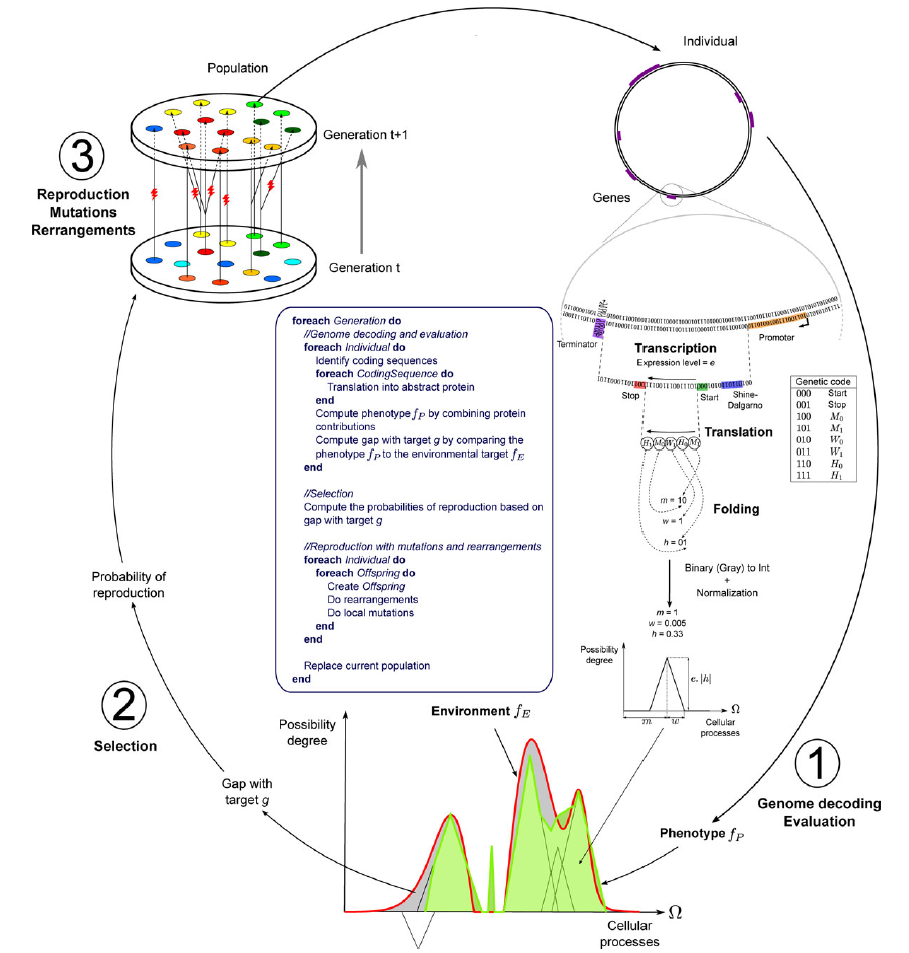
\includegraphics[scale=0.65]{aevol_overview01}
	\centering
	\caption[Overview of Aevol's architecture.]{Overview of Aevol's architecture, from \cite{Batut.2013}}
\end{figure}
\subsubsection{Decoding the Genome}
In aevol a genome consists of a string of binary characters where 0 is complementary to 1. Each organism in the clonal population has a double-stranded circular genome which is either generated randomly or which was provided as input. To decode the genome and produce the phenotype, the sequence is searched for transcribed regions. Transcribed regions are denoted by promoter and terminator sequences. The promoter sequence is a sequence whose Hamming distance $d$ is within $d_{max} = 4$ mismatches of the predefined consensus sequence $0101011001110010010110$. Terminators are sequences which can form a stem-loop structure with a stem size of 4 bases and a loop length of 3 bases. Lastly, the initiation and termination signals are sought, which are simply Shine-Dalgarno-like signals (i.e. $011011****000$ to start and $011011****001$ to stop). 

Once an initiation sequence is found, the following bases are read three at a time according to the genetic code given in Figure \ref{fig:aevol_overview01} until a stop codon (by default $001$) is found. These codons encode for three parameters, $M$ (mean), $W$ (half-width), and $H$ (height), which together define a triangle representing a "cellular process".

A cellular process is simply an abstract representation of some phenotypic function and is represented by the ordered set $\Omega = \left[0,1\right] \subset \mathbb{R}$. \textit{Fuzzy logic} is used to find the overall contribution of each cellular process. The mean $M$, then, gives us the specific cellular process, and is in the range $\left[0,1\right]$ The width describes the "scope" of the process, i.e. the \textit{pleiotropy} of the process. Lastly, the height determines the degree of possibility of the process, i.e. its relative strength. Since a transcribed region may have multiple initiation signals, codons are allowed.  

\subsubsection{Selection}
After the genome is decoded, the organisms are tested for their fitness. Fitness in Aevol is defined as the gap between the phenotype of a sequence and the environmental function $f_E$, as illustrated in Figure \ref{fig:aevol_overview01}. This environmental target function $f_E$ is a user-determined set of Gaussians which are specified in a parameter file. The difference between the phenotype (as calculated above) and the environmental function is the "metabolic error", labeled $g$ in the Figure. 

Aevol contains several selection schemes but here we will only consider the \texttt{fitness\_proportionate} scheme, since this was the only selection scheme employed in our experiments. In this scheme, the probability of reproduction for each organism is proportionate to its fitness, which is to say $exp(-k * g)$, where $k$ is a user-definable parameter which determines the selection intensity and $g$ is the metabolic error.
\subsubsection{Reproduction}

\subsection{aevol's Post-Treatments}\label{aevol_post-treatments}

\subsubsection{aevol\_misc\_ancestor\_mutagenesis}
This post-treatment generates and analyses mutants for the provided lineage. Specifically, this program generates evolvability, robustness, and antirobustness statistics for the mutants. 
\begin{enumerate}
	\item Generation
	\item Fraction of positive mutants
	\item Fraction of neutral mutants (reproductive robustness)
	\item Faction of neutral mutants (mutational robustness)
	\item Fraction of negative mutants
	\item Cumulative delta-gaps of positive mutants
	\item Cumulative delta-gaps of negative mutants
	\item Delta-gap for the best mutants
	\item Delta-gap for the worst mutant
	\item Cumulative delta-fitness of positive mutants
	\item Cumulative delta-fitness of negative mutants
	\item Delta-fitness for the best mutants
	\item Delta-fitness for the worst mutants
\end{enumerate}
\subsubsection{aevol\_misc\_ancestor\_robustness}
Generates mutants for a given lineage and analyzes their robustness, providing several statistics:
\begin{enumerate}
	
	\item Generation 
	\item Fraction of positive offspring 
	\item Fraction of neutral offspring (aka reproductive robustness) 
	\item Fraction of neutral mutants (aka mutational robustness) 
	\item Fraction of negative offspring 
	\item Cumulation of delta-gaps of positive offspring
	\item Cumulation of delta-gaps of negative offspring
	\item Delta-gap for the best offspring 
	\item Delta-gap for the worst offspring 
	\item Cumulation of delta-fitness of positive offspring 
	\item Cumum of delta-fitness of negative offspring
	\item Delta-fitness for the best offspring
	\item Delta-fitness for the worst offspring
\end{enumerate}


\subsubsection{aevol\_misc\_ancestor\_stats}

Analyzes a lineage and produces the following outputs:
\begin{enumerate}
	\item non-coding statistics (e.g. ancestor\_stats\_bp-b000000000-e000010000-i196-r1.out)
	\item mutation statistics (e.g. ancestor\_stats\_mutation-b000000000-e000010000-i196-r1.out)
	\item Each generation’s M W H (currently not working? – e.g. ancestor\_stats\_envir-b000000000-e000010000-i196-r1.out)
	\item Each generation’s genome size and termination number (e.g. ancestor\_stats\_nb\_term-b000000000-e000010000-i196-r1.out)
	\item The lineage’s fitness statistics
	\begin{enumerate}
		\item Generation
		\item Population size
		\item Fitness
		\item Genome size
		\item Metabolic error
		\item Parent’s metabolic error
		\item Metabolic fitness
		\item Secretion error
		\item Parent’s secretion error
		\item Secretion fitness
		\item Amount of compound present in the grid cell
		\item Int probe
		\item Double probe
		
	\end{enumerate}
	\item Statistics about the how many genes are in 20 RNA (e.g. ancestor\_stats\_operons-b000000000-e000010000-i196-r1.out)
	\item Individual gene statistics
	\begin{enumerate}
		\item Generation
		\item Number of coding RNAs
		\item Number of non-coding RNAs
		\item Average size of coding RNAs
		\item Average size of non-coding RNAs
		\item Number of functional genes
		\item Number of non-functional genes
		\item Average size of functional genes
		\item Average size of non-functional genes
	\end{enumerate}
	\item Rearrangement statistics (e.g. ancestor\_stats\_rear-b000000000-e000010000-i196-r1.out)
	\begin{enumerate}
		\item Generation
		\item Actual duplication rate
		\item Actual deletion rate
		\item Actual translocation rate
		\item Actual inversion rate
		\item Average alignment score
	\end{enumerate}
\end{enumerate}


\subsubsection{aevol\_misc\_coalescence}
Prints coalescence statistics for a given lineage.

\subsubsection{aevol\_misc\_create\_eps}
Creates a directory, analysis-generation\_XXXXX with several EPS files.The EPS files are as follows:
\begin{itemize}
	\item best\_genome\_with\_CDS.eps 
	\item best\_genome\_with\_mRNAs.eps
	\item best\_phenotype.eps
	\item best\_pos\_neg\_profiles.eps
	\item best\_triangles.eps
\end{itemize}

\subsubsection{aevol\_misc\_extract}

Extracts the genotype and/or data about the phenotype of individuals in the provided population and write them into text files for easy parsing by programs such as MATLAB. The program lets you specify whether you want the sequence, the triangle data, or both. By default (i.e. with no parameters) gives just the sequence, into a file called “sequence”.

\subsubsection{aevol\_misc\_lineage}

Using the tree files, recreates the lineage of an individual. By default, this is done for the best individual, but another individual can be specified by ID number or rank (-i or -r, respectively). 

\subsubsection{aevol\_misc\_mutagenisis}

This generates and analyzes mutations for an individual from a population backup (as opposed to a lineage file for ancestor\_mutagenesis). One can specify point mutations, small indels, duplications, large deletion, translocations, or inversions. 

\subsubsection{aevol\_misc\_protein\_map}

Creates a CSV file which analyzes the proteins generated by the specified lineage. The CSV file specifies:
\begin{enumerate}
	\item generation – Which generation is being described
	\item protein\_id – An identifier for the protein.
	\item shine\_dal – The location of the Shine-Dalgarno initiator for the protein
	 on the sequence.
	\item length – The number of base pairs which encodes the protein.
	\item concentration – The “amount” of a protein encoded, specified by the distance between the promoter and the consensus sequence. 
	\item hamming\_dist – The Hamming distance between the promoter sequence and the consensus sequence.
	\item dist\_next\_protein – The distance to the next protein?
	\item nb\_proteins – The number of proteins?
	\item dna\_length – The length of the DNA sequence.
\end{enumerate}


\subsubsection{aevol\_misc\_robustness}

Calculates replication statistics for a given individual (specified by either ID or rank) at a given time.  Specifically, the following information is saved in a new directory (analysis-generation\_XXXXXXXXXX):
\begin{enumerate}
	\item Parent id – The identifier of this organism’s parent.
	\item Parent metabolic error – The metabolic error rate of the parent.
	\item Parent secretion – The secretion rate of the parent.
	\item Mutant metabolic error – The metabolic error rate of the mutant.
	\item Mutant secretion – The secretion rate of the mutant.
	\item Mutant genome size – The genome size of the mutant.
	\item Mutant number of functional genes – The number of functional genes in the mutant.
\end{enumerate}

\section{Changeable Factors}
\subsection{Fitness}
\subsection{Evolvability}
\subsection{Robustness}
\subsection{Structure}
\subsubsection{Percent Coding vs. Non-Coding DNA}
\subsubsection{Number of Genes}


\section{Related Work}\label{related_work}
